\documentclass{beamer}
\usepackage[utf8]{inputenc}
\usepackage[squaren]{SIunits}
\usepackage{varwidth,setspace}
\usepackage{tikz}
\usetikzlibrary{intersections,positioning,backgrounds,fit,matrix,shapes,calc,decorations.pathmorphing}
\usetheme{default}

\setbeamertemplate{navigation symbols}{}%remove navigation symbols
\setbeamertemplate{footline}{\hspace*{.5cm}\scriptsize{\hfill\raisebox{1mm}{\insertframenumber}\hspace*{.5cm}}}

\setlength{\tabcolsep}{0.5mm}

\title{Measuring B-modes}
\author{Sigurd Kirkevold Næss}
\institute{Subdepartment of astrophysics, Oxford University}
\date{September 9th, 2014}

\begin{document}

\begin{frame}
	\titlepage
\end{frame}

\begin{frame}{From pristine CMB to dirty data}
	\begin{center}
		\large%
		\only<1>{At the surface of last scattering}%
		\only<2>{Lensing by large-scale structure}%
		\only<3>{Dusty galaxies, radio sources, SZ clusters}%
		\only<4>{Faraday rotation}%
		\only<5>{Galctic dust, synchrotron, etc}%
		\only<6>{Atmospheric emission}%
		\only<7>{Absolute polarization offset ($1^\circ$ example)}%
		\only<8>{Telescope optics (w. sidelobe)}%
		\only<9>{Detector noise}%
		\only<10>{Glitches}%
		\uncover<1-0>{()}% Dummy to keep line height constant
	\end{center}
	\begin{tikzpicture}[thick,red,decoration={snake, amplitude=1mm,segment length = 5mm}]
		\node at (0.0,0) (A) {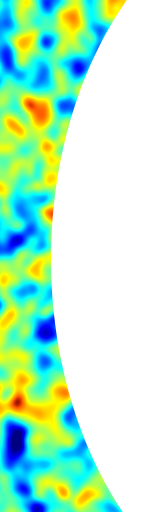
\includegraphics[height=1cm]{sls.png}};
		\node at (2.5,0) (B) {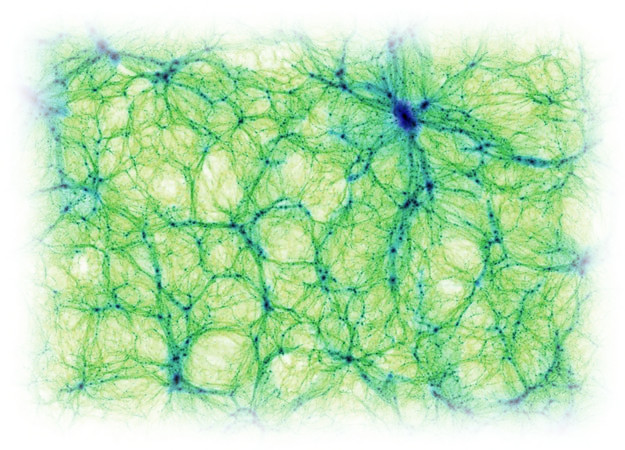
\includegraphics[height=1.5cm]{lss.jpeg}};
		\node at (5.0,0) (C) {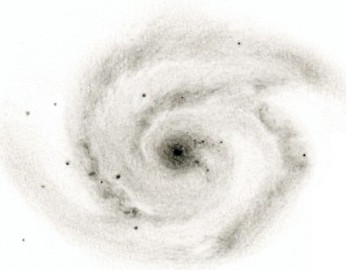
\includegraphics[height=1cm]{galaxy.jpeg}};
		\node at (7.5,0) (D) {
\includegraphics[height=1cm]{cloud.jpg}};
		\node at (10.0,0) (E) {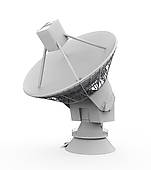
\includegraphics[height=1cm]{telescope.jpg}};
		\only<1>{\draw [decorate] (0,0) -- (0.5,0);}%
		\only<2-3>{\draw [decorate] (0,0) -- (2.5,0);}%
		\only<4-5>{\draw [decorate] (0,0) -- (5.0,0);}%
		\only<6>{\draw [decorate] (0,0) -- (7.5,0);}%
		\only<7-10>{\draw [decorate] (0,0) -- (10.0,0);}%
	\end{tikzpicture}
	\hspace*{-5mm}\begin{tabular}{ccc}
		T&E&B\\
	\only<1>{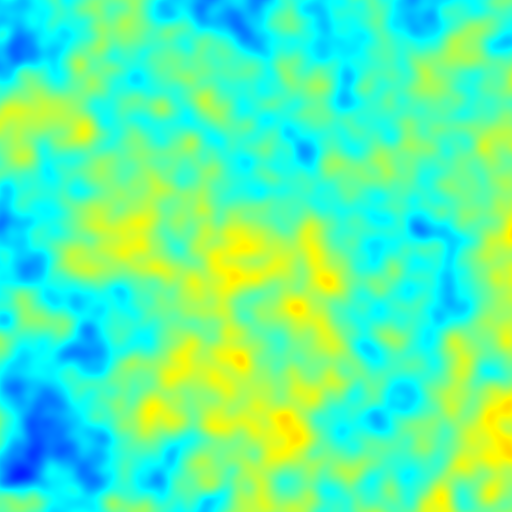
\includegraphics[width=0.35\textwidth]{out_dirty/01_cmb_teb_0.png}}%
	\only<2>{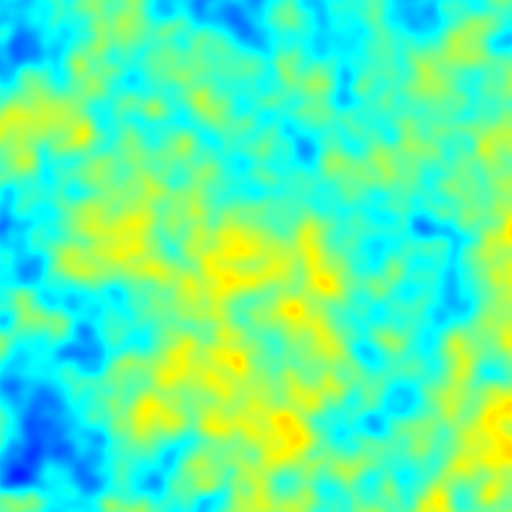
\includegraphics[width=0.35\textwidth]{out_dirty/02_lens_teb_0.png}}%
	\only<3>{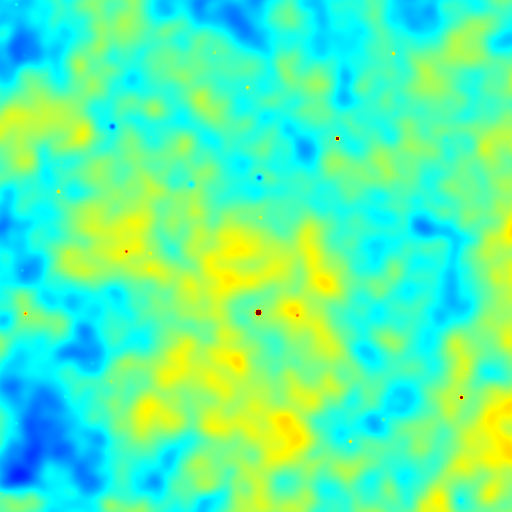
\includegraphics[width=0.35\textwidth]{out_dirty/04_sz_teb_0.png}}%
	\only<4>{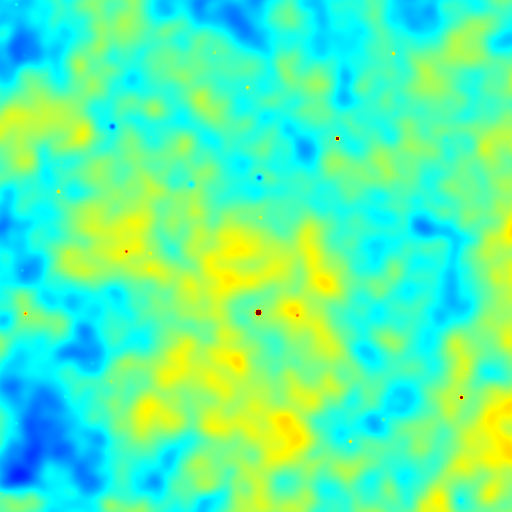
\includegraphics[width=0.35\textwidth]{out_dirty/05_faraday_teb_0.png}}%
	\only<5>{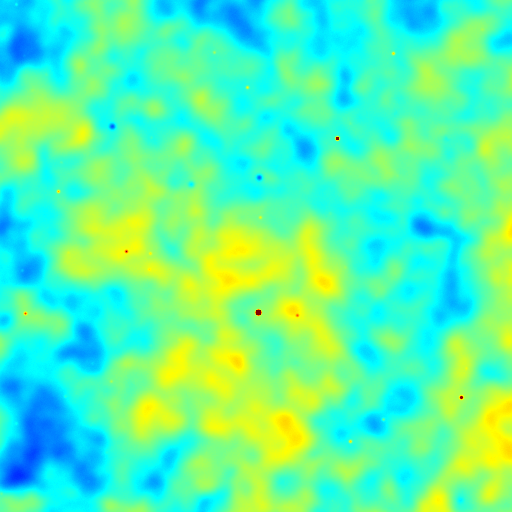
\includegraphics[width=0.35\textwidth]{out_dirty/06_dust_teb_0.png}}%
	\only<6>{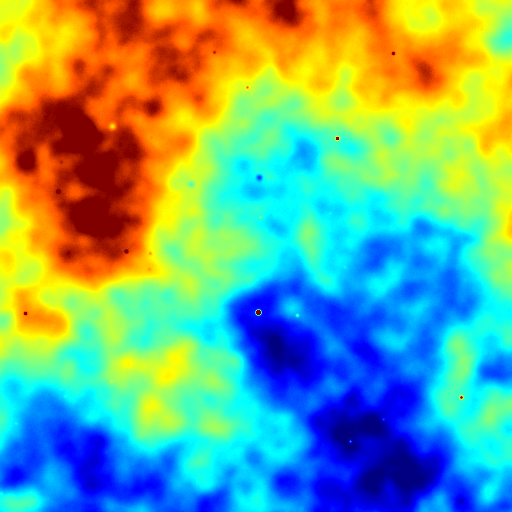
\includegraphics[width=0.35\textwidth]{out_dirty/07_atm_teb_0.png}}%
	\only<7>{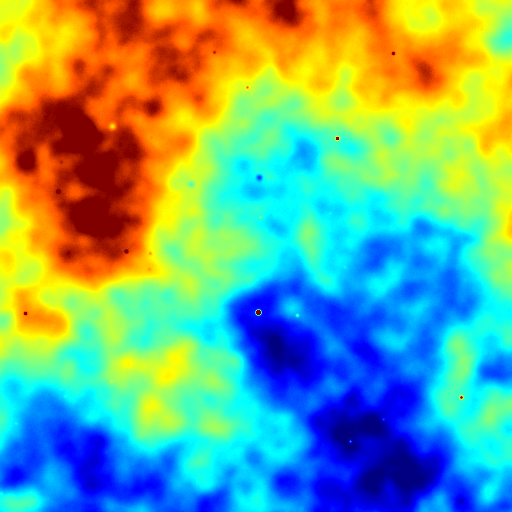
\includegraphics[width=0.35\textwidth]{out_dirty/08_polerr_teb_0.png}}%
	\only<8>{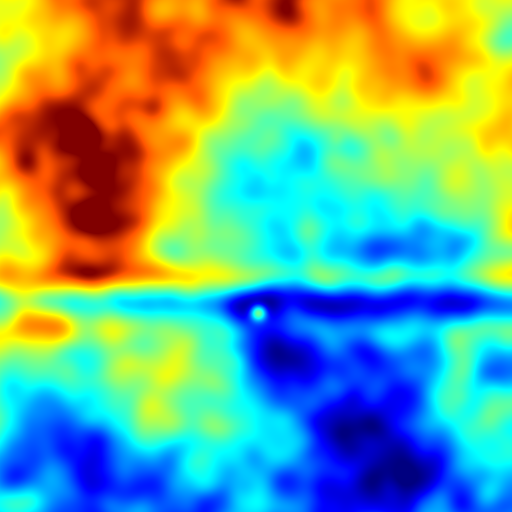
\includegraphics[width=0.35\textwidth]{out_dirty/10_beam_teb_0.png}}%
	\only<9>{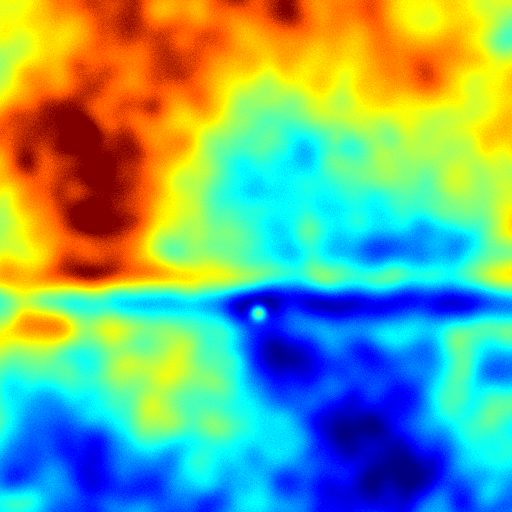
\includegraphics[width=0.35\textwidth]{out_dirty/11_noise_teb_0.png}}%
	\only<10>{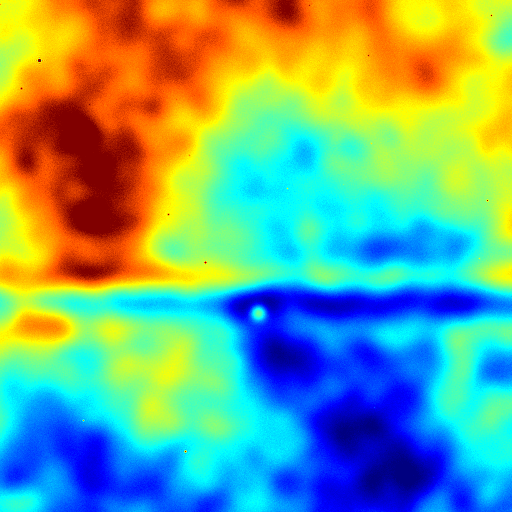
\includegraphics[width=0.35\textwidth]{out_dirty/12_glitch_teb_0.png}}%
	&
	\only<1>{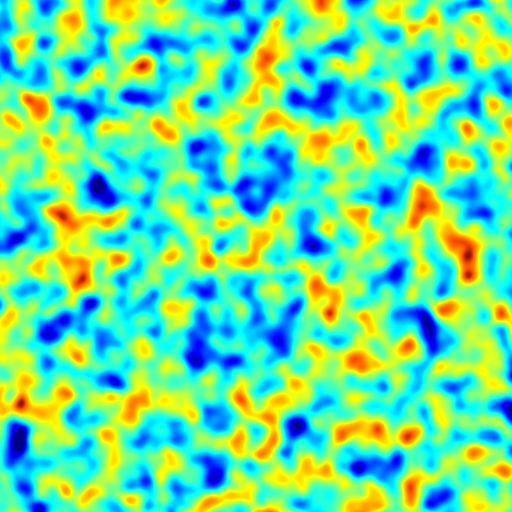
\includegraphics[width=0.35\textwidth]{out_dirty/01_cmb_teb_1.png}}%
	\only<2>{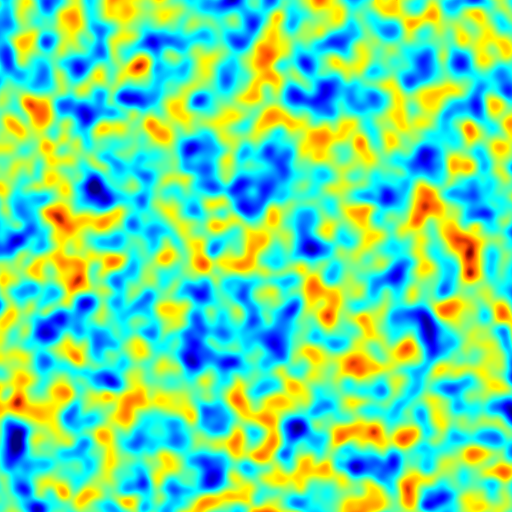
\includegraphics[width=0.35\textwidth]{out_dirty/02_lens_teb_1.png}}%
	\only<3>{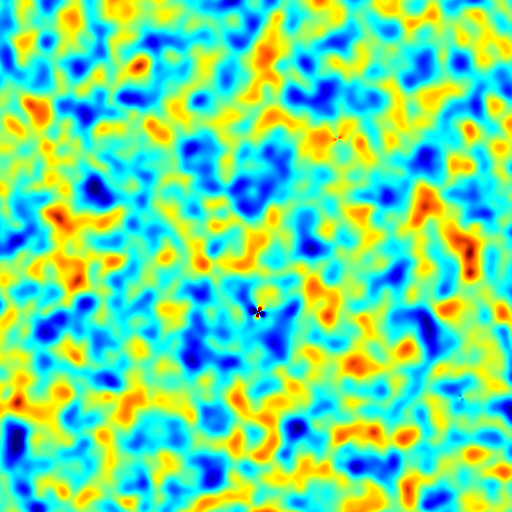
\includegraphics[width=0.35\textwidth]{out_dirty/04_sz_teb_1.png}}%
	\only<4>{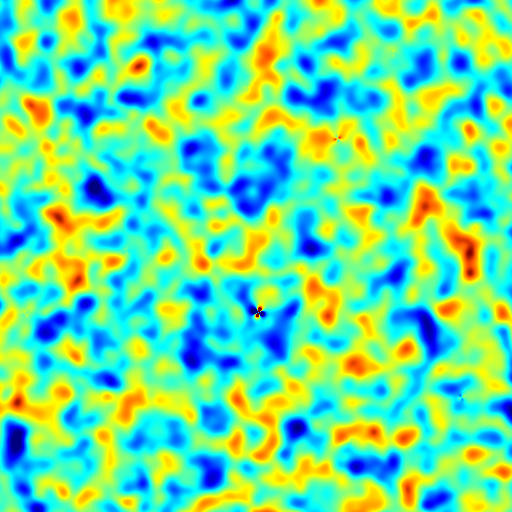
\includegraphics[width=0.35\textwidth]{out_dirty/05_faraday_teb_1.png}}%
	\only<5>{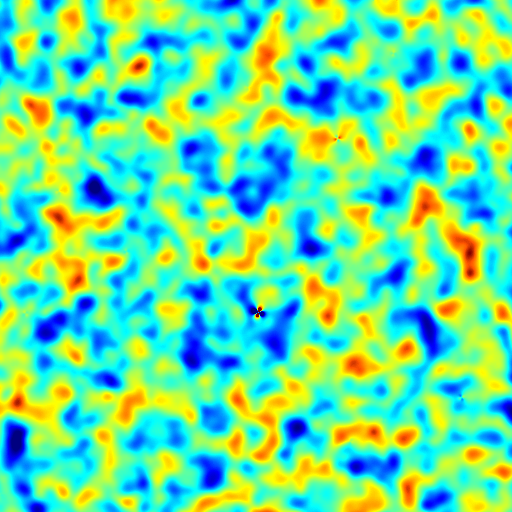
\includegraphics[width=0.35\textwidth]{out_dirty/06_dust_teb_1.png}}%
	\only<6>{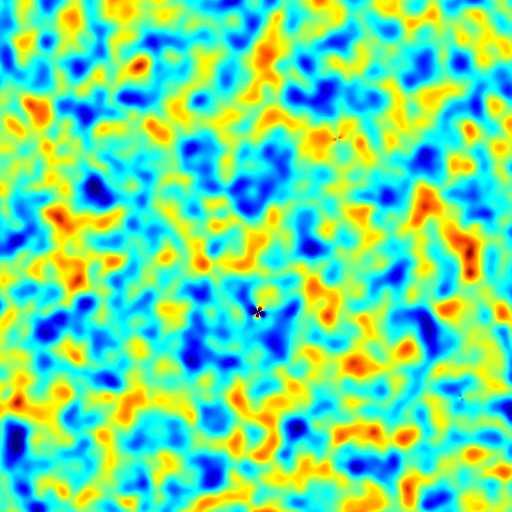
\includegraphics[width=0.35\textwidth]{out_dirty/07_atm_teb_1.png}}%
	\only<7>{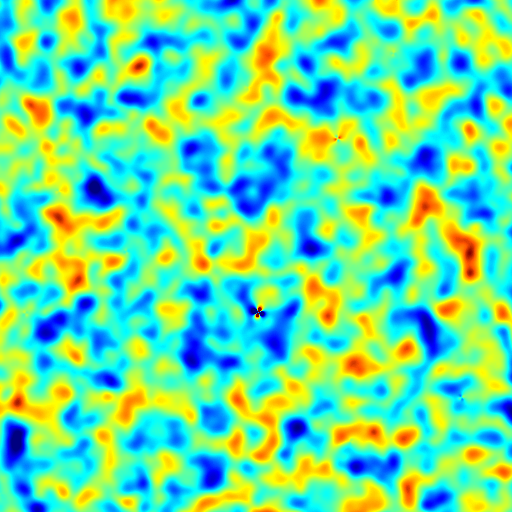
\includegraphics[width=0.35\textwidth]{out_dirty/08_polerr_teb_1.png}}%
	\only<8>{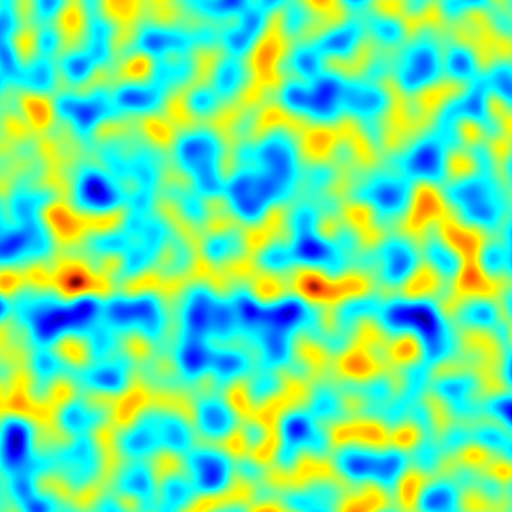
\includegraphics[width=0.35\textwidth]{out_dirty/10_beam_teb_1.png}}%
	\only<9>{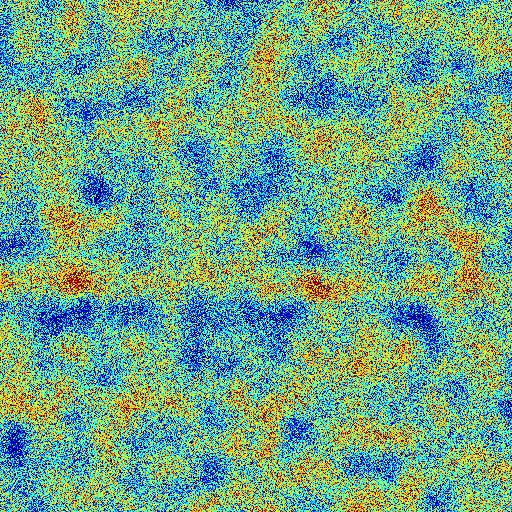
\includegraphics[width=0.35\textwidth]{out_dirty/11_noise_teb_1.png}}%
	\only<10>{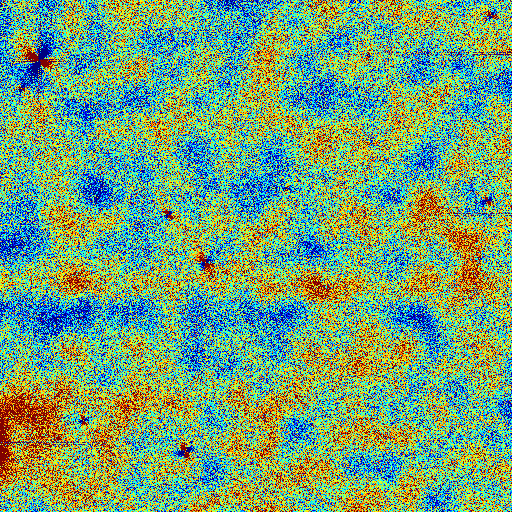
\includegraphics[width=0.35\textwidth]{out_dirty/12_glitch_teb_1.png}}%
	&
	\only<1>{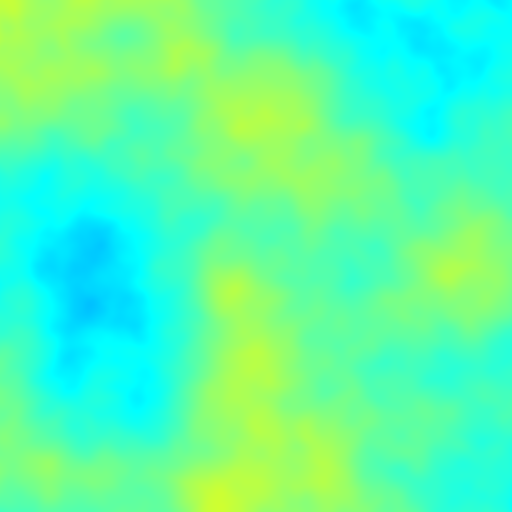
\includegraphics[width=0.35\textwidth]{out_dirty/01_cmb_teb_2.png}}%
	\only<2>{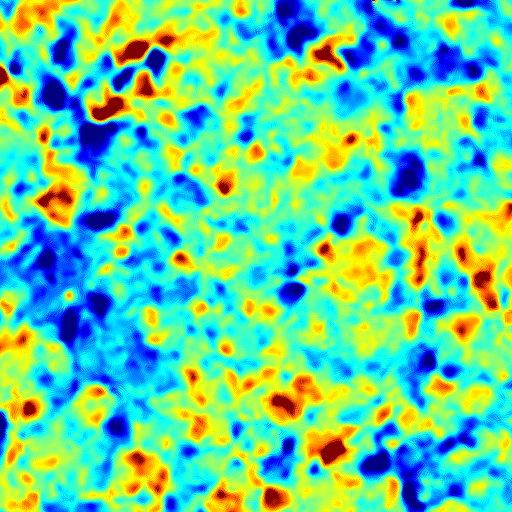
\includegraphics[width=0.35\textwidth]{out_dirty/02_lens_teb_2.png}}%
	\only<3>{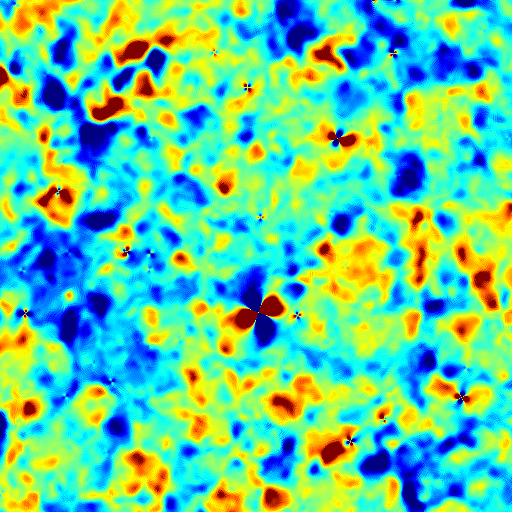
\includegraphics[width=0.35\textwidth]{out_dirty/04_sz_teb_2.png}}%
	\only<4>{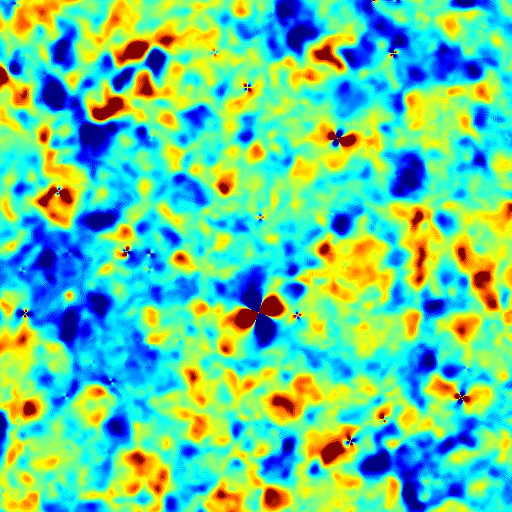
\includegraphics[width=0.35\textwidth]{out_dirty/05_faraday_teb_2.png}}%
	\only<5>{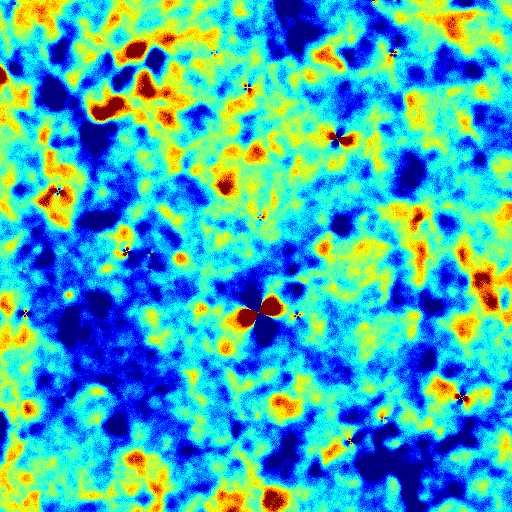
\includegraphics[width=0.35\textwidth]{out_dirty/06_dust_teb_2.png}}%
	\only<6>{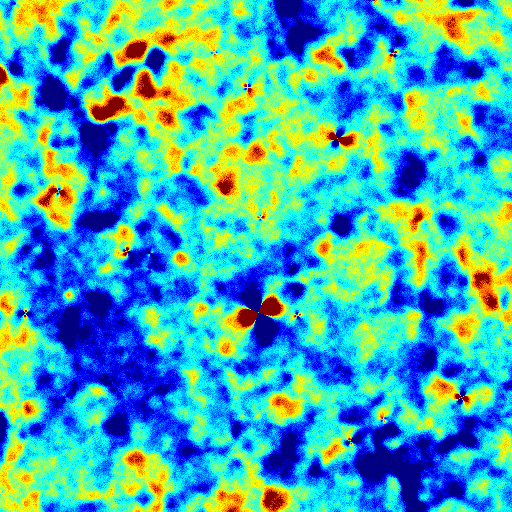
\includegraphics[width=0.35\textwidth]{out_dirty/07_atm_teb_2.png}}%
	\only<7>{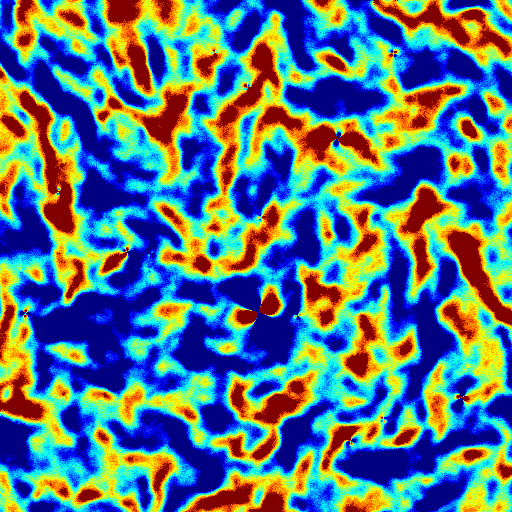
\includegraphics[width=0.35\textwidth]{out_dirty/08_polerr_teb_2.png}}%
	\only<8>{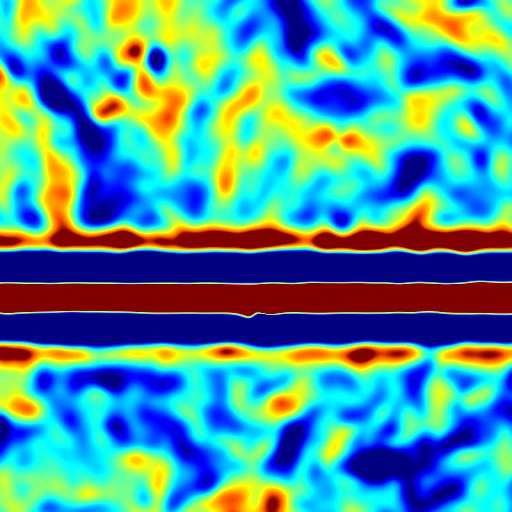
\includegraphics[width=0.35\textwidth]{out_dirty/10_beam_teb_2.png}}%
	\only<9>{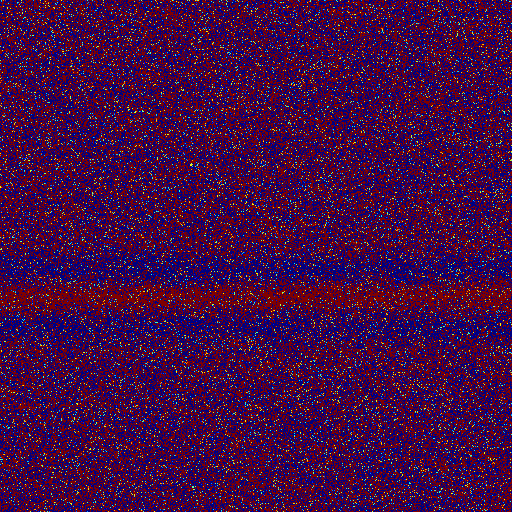
\includegraphics[width=0.35\textwidth]{out_dirty/11_noise_teb_2.png}}%
	\only<10>{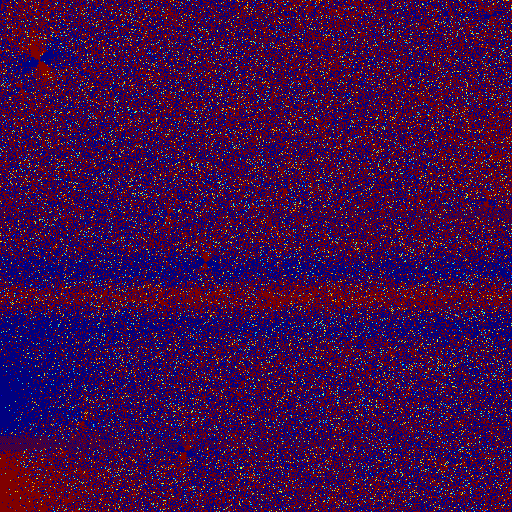
\includegraphics[width=0.35\textwidth]{out_dirty/12_glitch_teb_2.png}}%
	\\
	{\footnotesize $-500\mu$K\enskip
\includegraphics[width=12mm,height=2mm]{colorbar.png}\enskip$500\mu$K} &
	{\footnotesize $-20\mu$K\enskip
\includegraphics[width=12mm,height=2mm]{colorbar.png}\enskip$20\mu$K} &
	{\footnotesize $-1\mu$K\enskip
\includegraphics[width=12mm,height=2mm]{colorbar.png}\enskip$1\mu$K}
\end{tabular}\hspace*{-5mm}
\end{frame}

\begin{frame}{How the telescope actually observes}
	\begin{tikzpicture}[bad/.style={line width=8pt,red},scan/.style={thick,red}]
		\node at (0,0) (A) {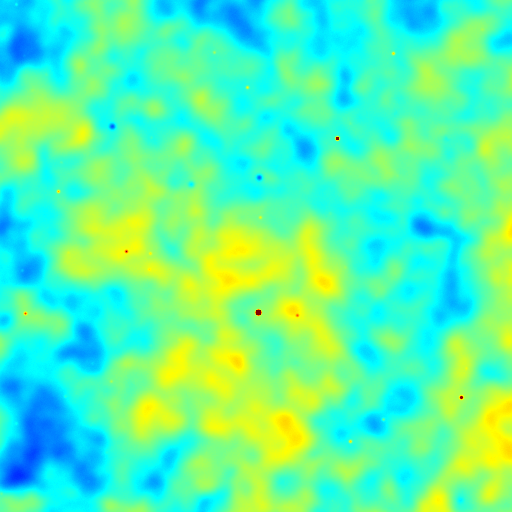
\includegraphics[height=3cm]{out_dirty/06_dust_teb_0.png}};
		\node at (1.5,-1) (B) {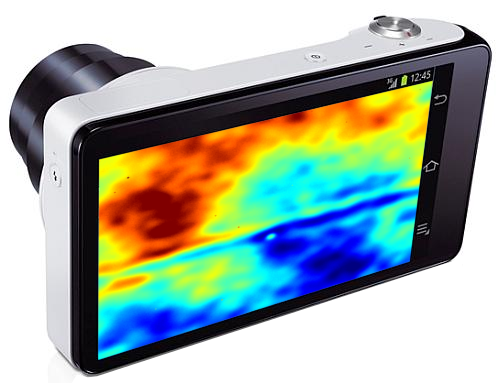
\includegraphics[height=3cm]{camera.png}};
		\draw[bad] (-1.1,-2.1) -- ( 2.6, 1.6);
		\draw[bad] (-1.1, 1.6) -- ( 2.6,-2.1);
		\uncover<2->{%
		\node at (6,0) (C) {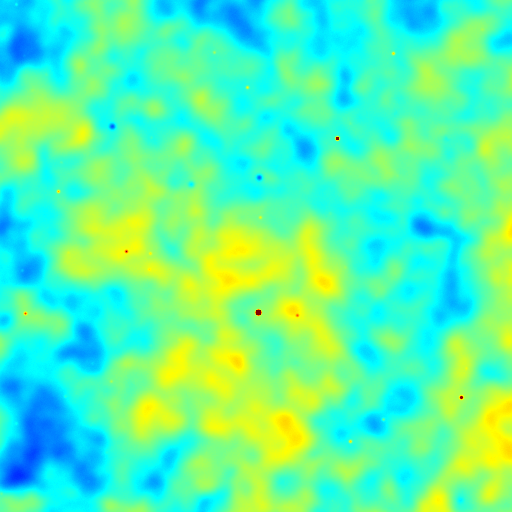
\includegraphics[height=3cm]{out_dirty/06_dust_teb_0.png}};}
		\uncover<3->{%
		\draw[scan] (5, 1.0) -- (7, 0.9);}
		\uncover<4->{%
		\draw[scan] (7, 0.9) -- (5, 0.8);}
		\uncover<5->{%
		\draw[scan] (5, 0.8) -- (7, 0.7);}
		\uncover<6->{%
		\draw[scan] (7, 0.7) -- (5, 0.6);}
		\uncover<7->{%
		\draw[scan] (5, 0.6) -- (7, 0.5);
		\draw[scan] (7, 0.5) -- (5, 0.4);
		\draw[scan] (5, 0.4) -- (7, 0.3);
		\draw[scan] (7, 0.3) -- (5, 0.2);
		\draw[scan] (5, 0.2) -- (7, 0.1);
		\draw[scan] (7, 0.1) -- (5, 0.0);
		\draw[scan] (5, 0.0) -- (7,-0.1);
		\draw[scan] (7,-0.1) -- (5,-0.2);
		\draw[scan] (5,-0.2) -- (7,-0.3);
		\draw[scan] (7,-0.3) -- (5,-0.4);
		\draw[scan] (5,-0.4) -- (7,-0.5);
		\draw[scan] (7,-0.5) -- (5,-0.6);
		\draw[scan] (5,-0.6) -- (7,-0.7);
		\draw[scan] (7,-0.7) -- (5,-0.8);
		\draw[scan] (5,-0.8) -- (7,-0.9);
		\draw[scan] (7,-0.9) -- (5,-1.0);
	\draw[scan] (5,-1.0) -- (7,-1.1);}
		\uncover<2->{
		\node at (7.5,-1) (D) {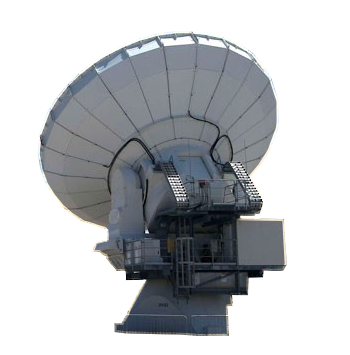
\includegraphics[height=3cm]{telescope2.png}};}
		\uncover<3->{%
		\draw[thick,red,->,rounded corners=1mm] (7.5,-2.4) -- (7.5,-2.6) -- (-0.5,-2.6) -- (-0.5,-2.9);
		\node at (-0.5,-3.00) {
\includegraphics[height=0.7mm,width=1.5cm]{out_dirty/scanrow100.png}};}
		\uncover<4->{%
		\node at ( 1.0,-3.00) {
\includegraphics[height=0.7mm,width=1.5cm]{out_dirty/scanrow116.png}};}
		\uncover<5->{%
		\node at ( 2.5,-3.00) {
\includegraphics[height=0.7mm,width=1.5cm]{out_dirty/scanrow132.png}};}
		\uncover<6->{%
		\node at ( 4.0,-3.00) {
\includegraphics[height=0.7mm,width=1.5cm]{out_dirty/scanrow148.png}};}
		\uncover<7->{%
		\node at ( 5.5,-3.00) {
\includegraphics[height=0.7mm,width=1.5cm]{out_dirty/scanrow164.png}};
		\node at ( 7.0,-3.00) {
\includegraphics[height=0.7mm,width=1.5cm]{out_dirty/scanrow180.png}};
		\node at (-0.5,-3.15) {
\includegraphics[height=0.7mm,width=1.5cm]{out_dirty/scanrow196.png}};
		\node at ( 1.0,-3.15) {
\includegraphics[height=0.7mm,width=1.5cm]{out_dirty/scanrow212.png}};
		\node at ( 2.5,-3.15) {\includegraphics[height=0.7mm,width=1.5cm]{out_dirty/scanrow228.png}};
		\node at ( 4.0,-3.15) {\includegraphics[height=0.7mm,width=1.5cm]{out_dirty/scanrow244.png}};
		\node at ( 5.5,-3.15) {\includegraphics[height=0.7mm,width=1.5cm]{out_dirty/scanrow260.png}};
		\node at ( 7.0,-3.15) {\includegraphics[height=0.7mm,width=1.5cm]{out_dirty/scanrow276.png}};
		\node at (-0.5,-3.30) {\includegraphics[height=0.7mm,width=1.5cm]{out_dirty/scanrow292.png}};
		\node at ( 1.0,-3.30) {\includegraphics[height=0.7mm,width=1.5cm]{out_dirty/scanrow308.png}};
		\node at ( 2.5,-3.30) {\includegraphics[height=0.7mm,width=1.5cm]{out_dirty/scanrow324.png}};
		\node at ( 4.0,-3.30) {\includegraphics[height=0.7mm,width=1.5cm]{out_dirty/scanrow340.png}};
		\node at ( 5.5,-3.30) {\includegraphics[height=0.7mm,width=1.5cm]{out_dirty/scanrow356.png}};
		\node at ( 7.0,-3.30) {\includegraphics[height=0.7mm,width=1.5cm]{out_dirty/scanrow372.png}};
		\node at (-0.5,-3.45) {\includegraphics[height=0.7mm,width=1.5cm]{out_dirty/scanrow388.png}};}
	\end{tikzpicture}
	\begin{center}
		\uncover<8->{\large Time-ordered data (TOD)}
	\end{center}
\end{frame}

\begin{frame}{The black magic of TOD analysis}
	\begin{itemize}
		\item Horribly noisy: S/N per sample of $\sim 10^{-4}$ for B-modes
		\begin{itemize}
			\item Compensate with lots of samples: $\sim 10^{12}$ typical
		\end{itemize}
		\item Full of systematic errors
			\begin{itemize}
				\item Instrument: beam, sidelobes, telephones, glitches, gain, pointing, cross-polarization, pol. angles, noise spectra, ...
				\item Sky: dust, synchrotron, free-free, point sources, faraday, lensing, zodiacal light, ...
			\end{itemize}
		\item Goal: Systematics-free high S/N CMB power spectrum
	\end{itemize}
\end{frame}

%\begin{frame}{From pristine CMB to dirty data}
%	\begin{itemize}
%		\item Surface of last scattering (young, enthusiastic photon)
%		\item Lensing by large-scale structure (+ISW)
%		\item Contaminated by dusty galaxies and radio sources
%		\item and distorted by the SZ effect
%		\item Enters our galaxy... (somewhat dirty and tired photon)
%		\item Contaminated by synchrotron, free-free and dust
%		\item and rotated and depolarized by magnetic fields
%		\item Enters solar system... (beat-up and messy photon)
%		\item Contaminated by Zodiacal light
%		\item Enters atmosphere...
%		\item Refracted
%		\item Contaminated by atmosphere (huge, but only T)
%		\item Enters telescope... (bleeding, crawling photon)
%		\item Contaminated by sun and ground from sidelobes
%		\item and optics polarization
%		\item and smeared by the beam (and pointing jitter)
%		\item Enters detector... (dead photon or electron)
%		\item Scaled by (uncertain, variable) gain
%		\item and smeared by (uncertain, variable) time constants
%		\item and contaminated by "1/f" and "white" noise (with uncertain, variable properties)
%		\item and data glitches
%		\item and rotated by uncertain detector polarization angles
%		\item The result: Time-ordered data
%		\item Task: Peel back all those layers of contamination to recover the pure CMB
%	\end{itemize}
%\end{frame}

\begin{frame}{Beating down the noise}
	\begin{itemize}
		\item Much of the contamination is noise. Array noise can be reduced by
			adding more detectors, and the rest can be integrated down by repeated
			observations.
		\item Scanning modulates signal, moving it from high-noise to lower-noise
			sample-frequencies.
		\item Results in very large data sets
		\item Map-making
	\end{itemize}
\end{frame}

\begin{frame}{Systematic effects}
	\begin{itemize}
		\item Do not automatically average down
		\item Must be modelled and removed or shown to be insignificant
		\item Split into telescope + sky systematics
	\end{itemize}
\end{frame}

\begin{frame}{Telescope systematics}
	\begin{itemize}
		\item Local effects from telescope or its local environment on Earth
		\item Glitches, seasonal/daily variations gain/pointing/beam, sun/ground sidelobes,
			magnetic pickup, instrument polarization, etc.
		\item Unlikely to rotate with the sky and have a fixed amplitude in sky-coordinates
		\item Will therefore vary depending on time and/or direction of observation
		\item Null tests: summer vs. winter, day vs. night, east vs. west, good vs. bad
			weather, high vs. low elevation, high vs. low scanning speed, etc.
		\item A good suite of null tests can make us confident that we have eliminated
			telescope systematics, and are seeing the sky as it is.
	\end{itemize}
\end{frame}

\begin{frame}{Sky systematics}
	\begin{itemize}
		\item Systematic effects between the Earth and the surface of last scattering
		\item Emission from the milky way (dust, synchrotron, etc.), faraday rotation,
			unresolved point sources, SZ clusters, lensing, etc.
		\item Fixed with respect to CMB
		\item but usually different spectrum: multi-frequency observations necessary
		\item Exception: lensing
	\end{itemize}
\end{frame}

\begin{frame}{Observational status}
	\begin{itemize}
		\item Before BICEP 2: Forest of measurements all fit standard 8-parameter(check)
			LCDM model with no tensor perturbations (r < 0.11)
		\item r limited by T cosmic variance
		\item B-modes do not suffer from this, but not competitive
		\item Lensing B-modes detected
		\item After BICEP 2: Solid detection at face value (5 sigma (check))
		\item Larger than expected
		\item Still very weak signal -> Have to worry about very weak systematics
	\end{itemize}
\end{frame}

\begin{frame}{BICEP 2 telescope systematics}
	\begin{itemize}
		\item Cite some criticism
		\item Quick summary of most important telescope systematics
		\item Null test suite: Very thorough, telescope systematics probably not an issue
			(after revised paper)
	\end{itemize}
\end{frame}

\begin{frame}{BICEP 2 sky systematics}
	\begin{itemize}
		\item Summary of sky systematics considered by BICEP 2 team (mostly dust)
		\item The foreground models used
		\item Criticism + later developments
		\item Did not allow for (quite large) uncertainty in polarization models
		\item Wrong polarization fraction
		\item Radio loops??
		\item Results suffer from being single-frequency (But BICEP 1)
	\end{itemize}
\end{frame}

\begin{frame}{Upcoming experiments}
\end{frame}

\begin{frame}{Direct detection?}
\end{frame}

\end{document}
